Målet med denne doktorgraden var todelt. Først var det å forstå hvilke strategier som var effektiv for å kjøre raskt på flater i slalåm, og forsøke å forstå mekanismene bak gjennom å utforske de kinematiske endringene som lå til grunn for pumping. Basert på dette arbeidet var det forsøke å forstå hvordan trenere og lærere best underviser for å lære disse strategiene best. Arbeidet er på denne måten med å belyse hvordan man jobber med utøvere på høyt nivå. Disse fire målene er listet opp under

\begin{enumerate}
    \item Å forstå hvilke strategier som gode utøvere oppnår best tid med på flater i alpint
    \item Å forstå de kinematiske endringene som ligger til grunn for pumpeteknikken
    \item Teste om trenere kan oppnå bedre løypesetting gjennom å bruke kontekstuell interference
    \item Teste om trenere kan instruere og bedre feedback gjennom reinforcement learnings
\end{enumerate}

\begin{figure}[H]
\centering
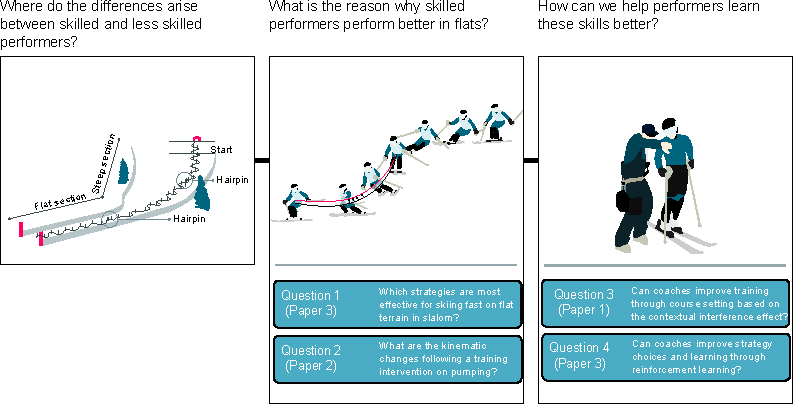
\includegraphics{figure_overview_3.pdf}
\caption{Kommer}
\label{fig:energy}
\end{figure}

